\chapter{Implementation and Results}
In this section we cover the implementation of the project and the results.
As outlined in the Objectives section we can divide the tasks into three main
parts: generation, transmission, and reception. 
In this project we looked at using a FPGA board for the generation and
reception of the PRBS data.  Hence the overall design is of a board in a
loopback configuration as shown in Figure~\ref{fig:loopback}.

\begin{figure}[ht]
    \centering
    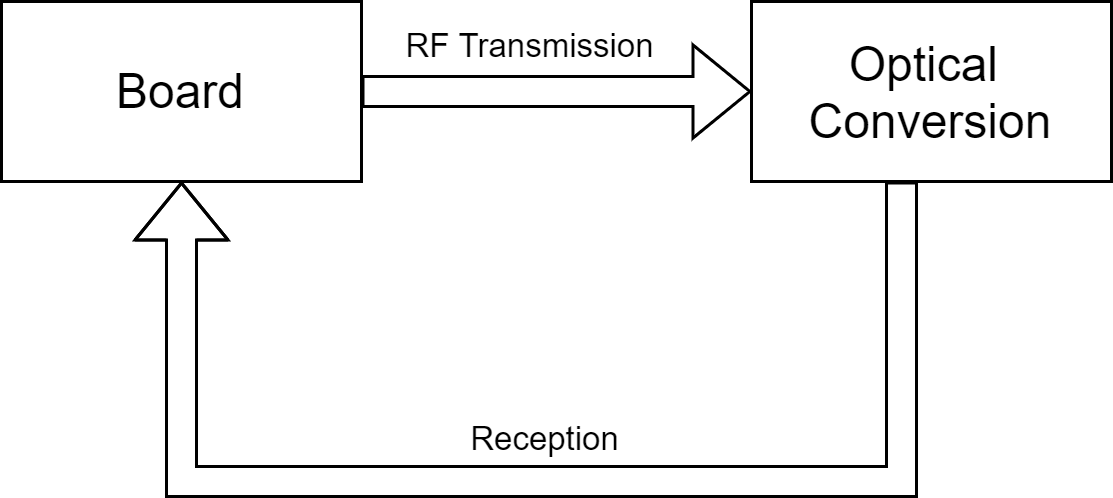
\includegraphics[width=0.6\linewidth]{img/loopback.png}
    \caption{Loopback Configuration}%
    \label{fig:loopback}
\end{figure}

\section{Generation and Reception}%
\label{sec:generation_and_reception}


\subsection{Hardware}%
\label{sub:hardware}
To generate and receive PRBS data the VCU118 board was used. To transmit the
data the board's internal high-speed parallel to serial GTY transceivers in
conjuction with a Si5345 external clock (as the board is not able to generate
an internal clock to the needed precision) were used.

\begin{figure}[ht]
    \centering
    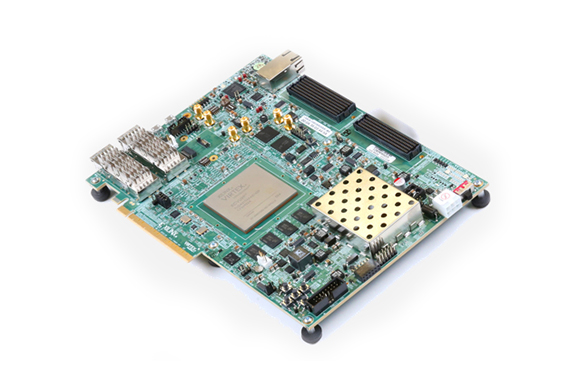
\includegraphics[width=0.5\linewidth]{img/board.jpg}
    \caption{VCU118 Board}%
    \label{fig:board}
\end{figure}

\begin{figure}[ht]
    \centering
    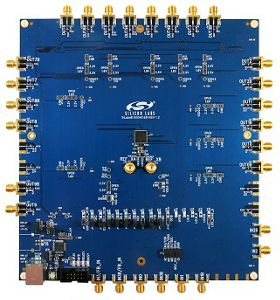
\includegraphics[width=0.4\linewidth]{img/clock.jpg}
    \caption{Si5345 Clock}%
    \label{fig:clock}
\end{figure}

\subsection{PRBS Generation}%
\label{sub:prbs_generation}

We looked to modify the functionality of a basic implementation of the
transceiver. In the basic implementation a PRBS generator is is fed to the
transceiver channel, through a wrapper. 

The PRBS module was unchanged from the default with the exception of reduced
the length of the PRBS sequence from PRBS31 (2.1 billion bits) to PRBS7 (511
bits) for ease of checking.
\subsubsection{Burst Mode over Single Channel}%
\label{ssub:burst_mode_over_single_channel}
and we set it to output zeros if the output flag was disabled.

\subsubsection{Switching Between Two Channels}%
\label{ssub:switching_between_two_channels}
The main modification was to change the PRBS wrapper to feed the two different
channels. Using a 2 bit register, the wrapper alternated between the two
channels as approrpriate.



\subsection{PRBS Checking}%
\label{sub:prbs_checking}

\subsubsection{Locking to Refrence Clock}%
\label{ssub:locking_to_refrence_clock}

\subsubsection{Burst Mode Checking}%
\label{ssub:burst_mode_checking}

\section{Optical Transmission}%
\label{optical_transmission}

\subsection{SOA Board}%
\label{sub:soa_board}

\subsection{Heatsink and Mount}%
\label{sub:heatsink_and_mount}





